\section{Results}
\label{sec:results}

%\emph{Benchmarks (test results) and possibly competition results.  Include explanations and analyses of your results. As mentioned under “Benchmarks and comparisons” below, it is usually a clear strength if you have some results to com- pare, e.g. two different versions of your client with different methods/features/parameters.  You could also compare the behaviour of your client on different individual levels that illustrate a certain point, e.g. similar levels resulting in large differences in the client’s behaviour.}

To showcase how efficient our goal prioritisation technique is and how we have improved upon it throughout the project, we present our client's solutions of the level \texttt{SAOptimal} with different goal prioritisation technique.
In the following we will refer to our main goal prioritisation technique (\cref{methods:goal_ordering}) as the ``complex'' prioritisation, and the ``simple'' differs in that it does not perform the final matrix computation as presented in \cref{methods:goal_ordering}.

The simple goal prioritization will use the first step of the goal prioritization technique described in \cref{methods:goal_ordering}. 
This will prioritize the goals placed in dead-ends or corners, higher than goals with adjacent free cells or other goal cells.

The problem with this technique can be seen in \cref{fig:simple priority}. 
The goals r and s, will have the same priority because they both have 3 goal cells and a wall adjacent to them. 
Therefore, the AI might pick r before s, causing s to be blocked off. 
The agent will then have to move the R box again in order to place the S box in the s goal causing an increase in actions taken.

% Example of cells 
\begin{figure}[h!]
  \centering
  \begin{minipage}{.45\columnwidth}
    \centering
    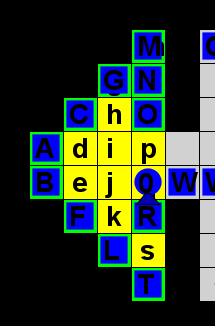
\includegraphics[height=5cm]{graphics/simple_priority_block.PNG}
    \caption{\label{fig:simple priority}Simple goal prioritisation.}
  \end{minipage}%
  \hspace{20pt}%
  \begin{minipage}{.45\columnwidth}
    \centering
    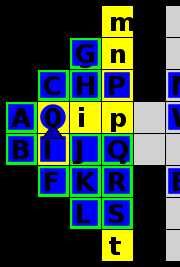
\includegraphics[height=5cm]{graphics/no_priority_block.png}
    \caption{\label{fig:no priority}No goal prioritisation.}
  \end{minipage}
\end{figure}

This is fixed in the complex goal prioritization, where the AI is told to choose the exact order in which the goals are prioritized, placing goals that will be blocked off higher than then goals that will block them.  
The improvements from the simple to the complex goal prioritization is illustrated in \cref{tab:SAOptimal_results}, where the results of the two runs are shown.

\begin{table}[h!]
  \centering
  \caption{\label{tab:SAOptimal_results}No. actions performed on \texttt{SAOptimal} level with different prioritisation techniques.}
  \begin{tabular}{@{}ll@{}}
    \toprule
    Prioritisation technique & Actions \\ 
    \midrule
    None    & $>1400$ \\ 
    Simple  & $761$ \\ 
    Complex & $730$ \\
    \bottomrule
  \end{tabular}
\end{table}

\subsection{Performance vs. Optimality}
\label{sec:performance vs. optimality}

We have developed a client with performance in mind.
The only technique we used to give better results was to develop the goal prioritisation technique, so the client did not fill in goals arbitrarily.
For course's competition presentation we found that, as an example, our client was beaten in \texttt{SAOptimal} with 7 \% less actions performed. 
However, our client solved the level approximately 700 times faster than the opponent.

Note that we performed our tests on a laptop with Intel® Core™ i5 4210U Processor (1.7 - 2.7 GHz), 4GB DDR3L 1600 MHz SDRAM, with an SSD hard drive.
